\subsection{UCP}
\label{sec:algorithms:ucp}

Utility Cache Partition~\cite{Qureshi2006} (UCP) was first presented by M. Qureshi and Y. Patt in 2006. 
UCP uses the concept of utility when assigning ways to a core.
Using a utility monitor (UMON), UCP calculates the number of ways assigned to each core.
UCP then uses the same insertion and promotion policy as LRU.
The replacement policy is as in LRU with two modifications:
First if the number of blocks owned by the requesting core is less than the number of ways assigned to it, then the least recently used block that is not assigned to the requester core is replaced.
If however the number of blocks owned is greater than or equal to the number of assigned ways the replacement algorithm selects the  least recently used block of those owned by the requester.
As a result, the division between cores in each set move towards the global allocation on cache misses, allowing cores to use more than allocated if other cores do not utilize their allocated space.

The UMON is the core of the UCP algorithm.
It consists of one ATD per core sharing the cache. 
The ATD is managed by normal LRU replacement and has one access counter per way.
Whenever a cache request hits in the ATD the access counter index by the LRU stack position of that block is incremented.
In other words, UMON uses the stack property of LRU to find the hit rate of all valid partition sizes.
In addition to the ATDs, there is a monitor circuit that has access to the counters and using them calculates how to partition the cache at set intervals. 
In the original paper, the authors recalculate the partitioning every 5M cycles.

The original paper proposes several algorithms for determining optimal partitioning based on the counter data. 
Algorithm~\ref{alg:algorithms:ucp} is the Lookahead Algorithm they propose.
This algorithm is the one the original authors propose for situations with more than two cores sharing a cache.
The algorithm assigns cache ways based on an increase in marginal utility.
While there are more ways to distribute, the algorithm calculates the maximum marginal utility achievable by each core. 
The core with the highest value wins and is assigned as many ways as needed to achieve the increase.
The algorithm continue until all ways have been assigned.
Lines 27-28 calculate the actual marginal utility. 
First the number of misses prevented by increasing the allocation from a to be is found.
With the counters available the algorithm can simply sum the values of counters a to $b-1$, as the number of hits in the new sets must equal the number of misses prevented.
To find the marginal utility, this value is then divided by the number of sets introduced.
The rest of the algorithm is simply a greedy algorithm selecting the best core each iteration.
After a reallocation of cache ways, the ATD counters are all halved.
By doing this, the UMON will keep historical data for future decisions, while prioritizing data from the current period.

\begin{figure}[ht]
    \centering
    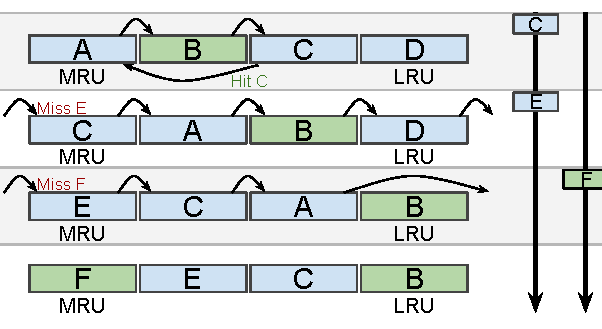
\includegraphics[width=.65\textwidth]{figures/algorithms/UCP}
    \caption[UCP managed 4-way cache set.]{UCP managed 4-way cache set. (Two cores each allocated two blocks)}
    \label{fig:algorithms:ucp_example}
\end{figure}

\begin{algorithm}[ht]
\caption{UMON Lookahead Algorithm.}
\label{alg:algorithms:ucp}
\begin{algorithmic}[1]
\State $balance\gets N$ /* Number of ways */
\State $allocations[i]\gets 0$  /* for each core $i$ */
\While {$balance$}
    \ForAll {$cores\ i$}
        \State $alloc\gets allocatations[i]$
        \State $max\_mu[i]\gets \Call{get\_max\_mu}{i, alloc, balance}$
        \State $blocks\_req[i]\gets$ min blocks to get max\_mu[i] for i
    \EndFor
    \State $winner\gets$ application with the maximum value of max\_mu
    \State $allocations[winner] += blocks\_req[winner]$
    \State $balance -= blocks\_req[winner]$
\EndWhile
\State \Return alloactions
\State

\Function{get\_max\_mu}{$i, alloc, balance$}
    \State $max\_mu\gets 0$
    \For{ii = 1; ii <= balance; ii++}
        \State $mu\gets \Call{get\_mu\_value}{p, alloc, alloc+ii}$
        \If{$mu \ge max\_mu$}
            \State $max\_mu\gets mu$
        \EndIf
    \EndFor
    \State \Return{$max\_mu$}
\EndFunction
\State

\Function{get\_mu\_value}{$p, a, b$}
    \State $U\gets$ change in misses for application p when number of blocks assigned to it increases from a to b
    \State \Return{$\frac{U}{b-a}$}
\EndFunction
\end{algorithmic}
\end{algorithm}
